\documentclass[12pt,a4paper]{book}
\usepackage[utf8]{inputenc}
\usepackage{amsmath}
\usepackage{amsfonts}
\usepackage{amssymb}
\usepackage{graphicx}
\usepackage[left=0.50cm, right=0.50cm, top=0.50cm, bottom=0.50cm]{geometry}
\author{Michael Schoderer}
\title{Architektur-Beschreibung: Bookstore}
\begin{document}
	\chapter{Bookstore}
	\section{Beschreibung}
	Die Java-EE Anwendung 'Bookstore' wurde für die Vorlesung Implementierung von Informationssystemen an der Technischen Hochschule Ingolstadt entwickelt und ermöglicht das Speichern und Verwalten von Dokumenten (PDF, MOBI, TXT, ...).
	\section{Architektur der Anwendung}
	\subsection{Übersicht}
	Bei der Konzeption und Entwicklung wurde die Anwendung in die im folgenden aufgelisteten Schichten unterteilt:
	\begin{itemize}
		\item \textbf{GUI} Die Oberfläche wurde mithilfe von JavaServer Faces (JSF) umgesetzt. Bei der Gestaltung der Oberfläche wurden Templates eingesetzt, damit ein einheitliches Bild der einzelnen Webseiten gewährleistet werden kann
		\item \textbf{Geschäftslogik} Die Geschäftslogik wurde unabhängig von der graphischen Oberfläche entwickelt, um eine Trennung nach dem MVC-Model zu erreichen
		\item \textbf{Datenbank} Die Datenbankschicht wurde durch mehrere Interfaces gekapselt und stellt die benötigten Funktionen bereit, um die Domain-Objekte zu in die jeweilige Datenbank zu persistieren		
		\end{itemize}
		
		
		
		
		\subsection{Package-Struktur}
		\begin{center}
		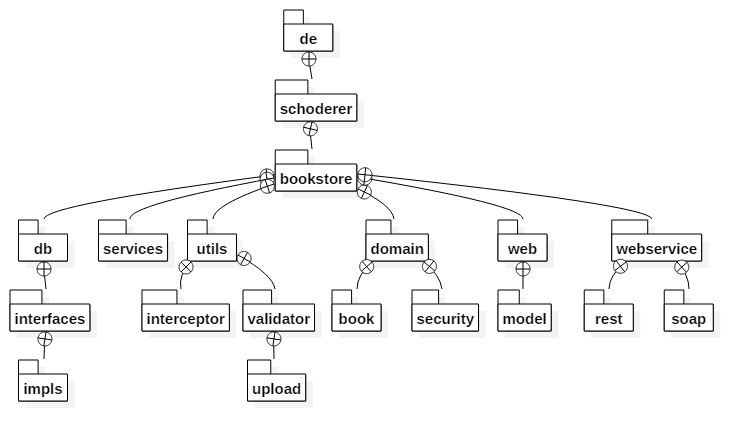
\includegraphics[width=1\textwidth]{Images/package.png}
		\label{fig1}
	\end{center}
	\underline{\textbf{Beschreibung der Packages}}
		\begin{description}
			\item[bookstore] \hfill \\
			 Dies ist das Hauptpackage der Anwendung
			 	\item[db.interfaces] \hfill \\
				 	Hier liegen die Interfaces, welche die Datenbankverbindungen abkapseln
			 		\item[db.interfaces.impls] \hfill \\
			 		Hier liegen die Implementierungen der Interfaces, welche konkrete Verbindungen zu einer spezifischen Datenbank aufbauen
			 	\item[services] \hfill \\
			 	In diesem Package befinden sich die Service-Klassen, welche die Geschäftslogik der Anwendung beinhalten
		\item[utils.interceptor] \hfill \\
		Die Interceptoren befinden sich in diesem Package
		\item[utils.validator] \hfill \\
		In diesem Package und dem Unterpacket "upload" befinden sich die JSF-spezifischen Validatoren, welche Usereingaben validieren
		\item[domain.book] \hfill \\
		Hier befinden sich die Domänenobjekte, welche für den Betrieb der Anwendung benötigt werden 
		\item[domain.security] \hfill \\
		Hier befinden sich die Domänenobjekte, welche die Benutzer und deren Rechte repräsentieren
		\item[web.model] \hfill \\
		In diesem Packet befinden sich die JSF-Beans
		\item[webservice.rest] \hfill \\
		Hier befinden sich die Klassen, die benötigt werden um die REST-API der Anwendung bereitzustellen
		\item[webservice.soap] \hfill \\
		Hier befinden sich die Klassen, die benötigt werden um die SOAP-API der Anwendung bereitzustellen
		\end{description}
		
		\subsection{Datenbank}
			\begin{center}
				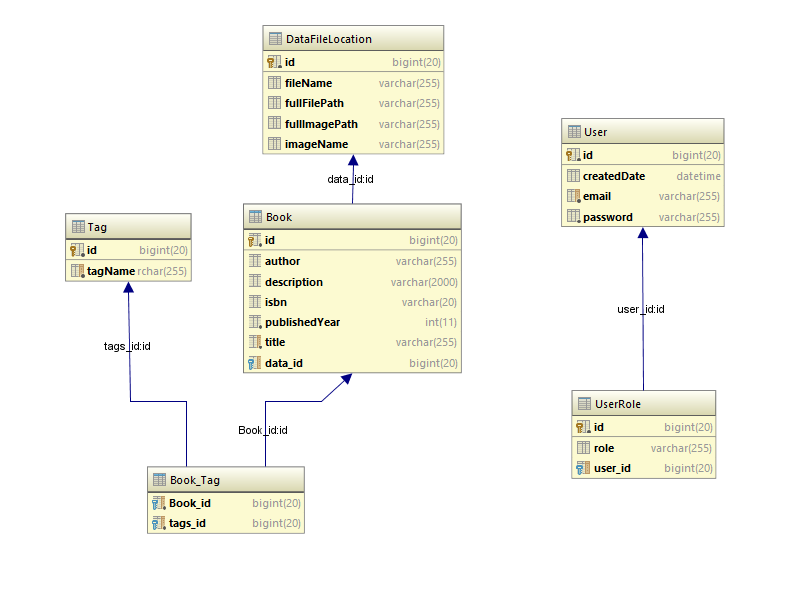
\includegraphics[width=0.8\textwidth]{Images/database.png}
				\label{fig2}
			\end{center}
		
			
		
		
\end{document}